% !TEX root = cha-implementation.tex
\documentclass[../../main.tex]{subfiles}

\begin{document}

\section{Tool}
\label{sec:tool}

To make \wassis easier to use and to inspect the generated visualizations, we developed a GUI in the Pharo environment. This section describes the main parts of the tool, including class selection, configuration, the main and additional visualizations.

\subsection{Class Selection and Config Setup}

The procedure starts with the panel shown in \figref{fig:class_selection}. Here, users can search and select a class or component from the target system. They can also choose which relationships to visualize and set the number of instances to run in parallel.

\begin{figure}[ht]
    \centering
    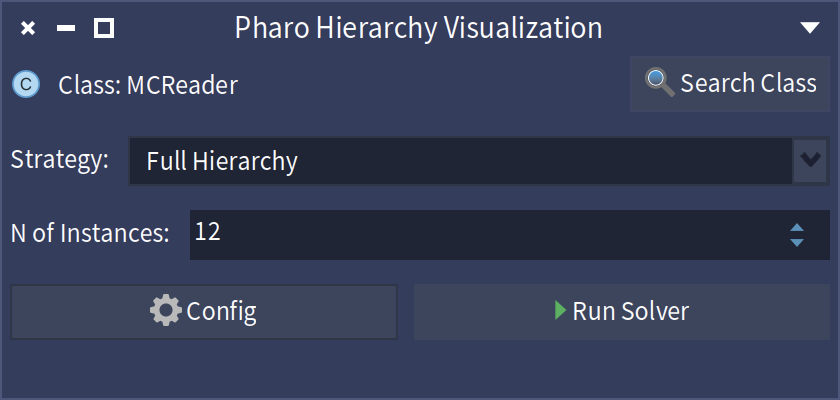
\includegraphics[width=0.80\textwidth]{figures/implementation/tool/class_selection}
    \caption{\wassis visualization configuration}
    \label{fig:class_selection}
\end{figure}

The \texttt{Config} button opens the settings window shown in \figref{fig:config_window}. The settings are divided into four groups:

\begin{itemize}
    \item \textbf{General Configuration:} Controls the heap type, the class placement order, and the minimum desired distance between classes.
    
    \item \textbf{Path Configuration:} Sets the exit assignment strategy for the class footprints and the boost value applied to all path directions.
    
    \item \textbf{Tile Weights:} Sets the weights for empty, straight, and corner tiles.
    
    \item \textbf{Backtracking Configuration:} Sets the retry limits for backtracking on the same graph, same class placement, and same grid size. It also provides different backtracking strategies and their specific parameters.
\end{itemize}

\begin{figure}[ht]
    \centering
    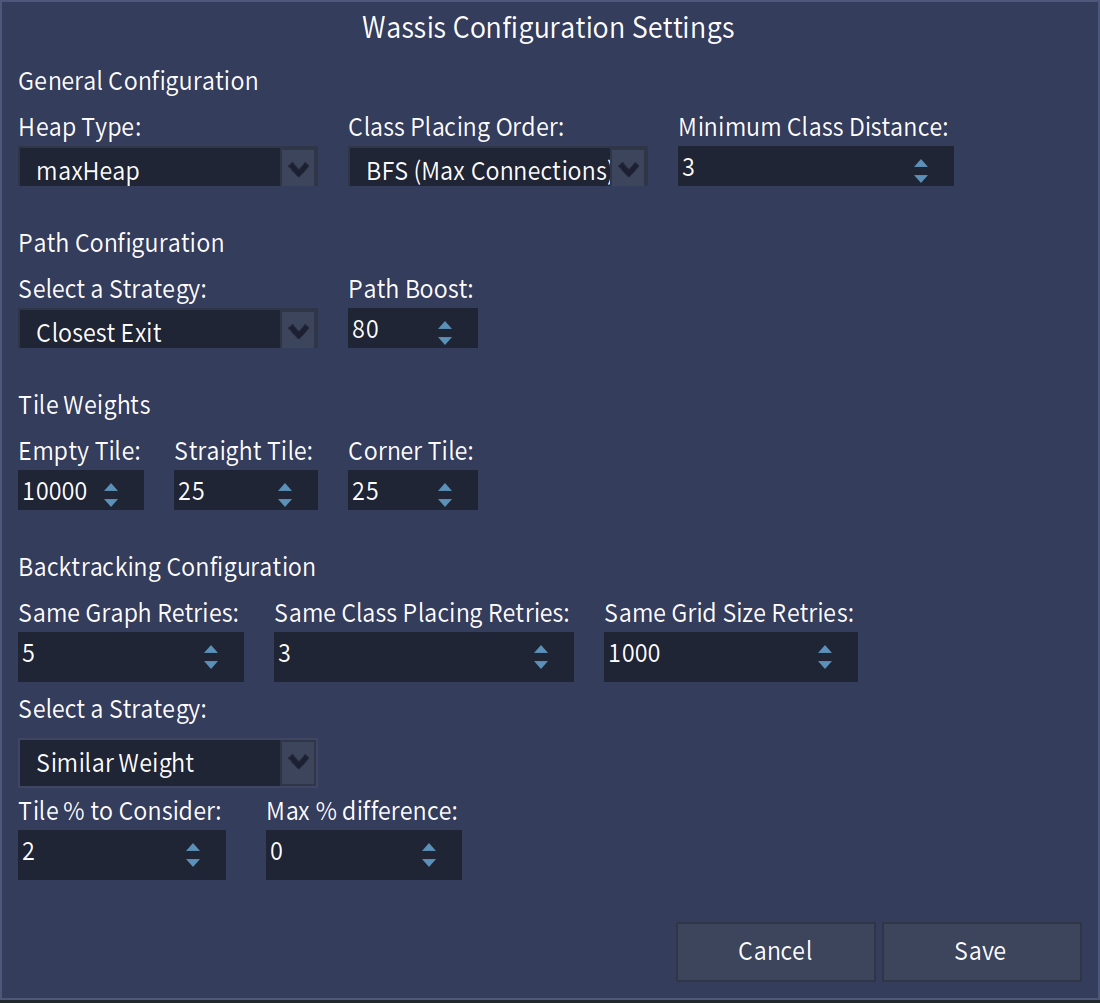
\includegraphics[width=0.85\textwidth]{figures/implementation/tool/config_window}
    \caption{\wassis configuration settings window.}
    \label{fig:config_window}
\end{figure}

\subsection{Visualization and Additional Views}

Once a valid solution is found, \wassis displays the generated 2D visualization on an interactive canvas using Roassal (\figref{fig:visualization}). Users can inspect the objects using the Pharo Inspector, save the solution using Fuel, and open additional views.

\begin{figure}[ht]
    \centering
    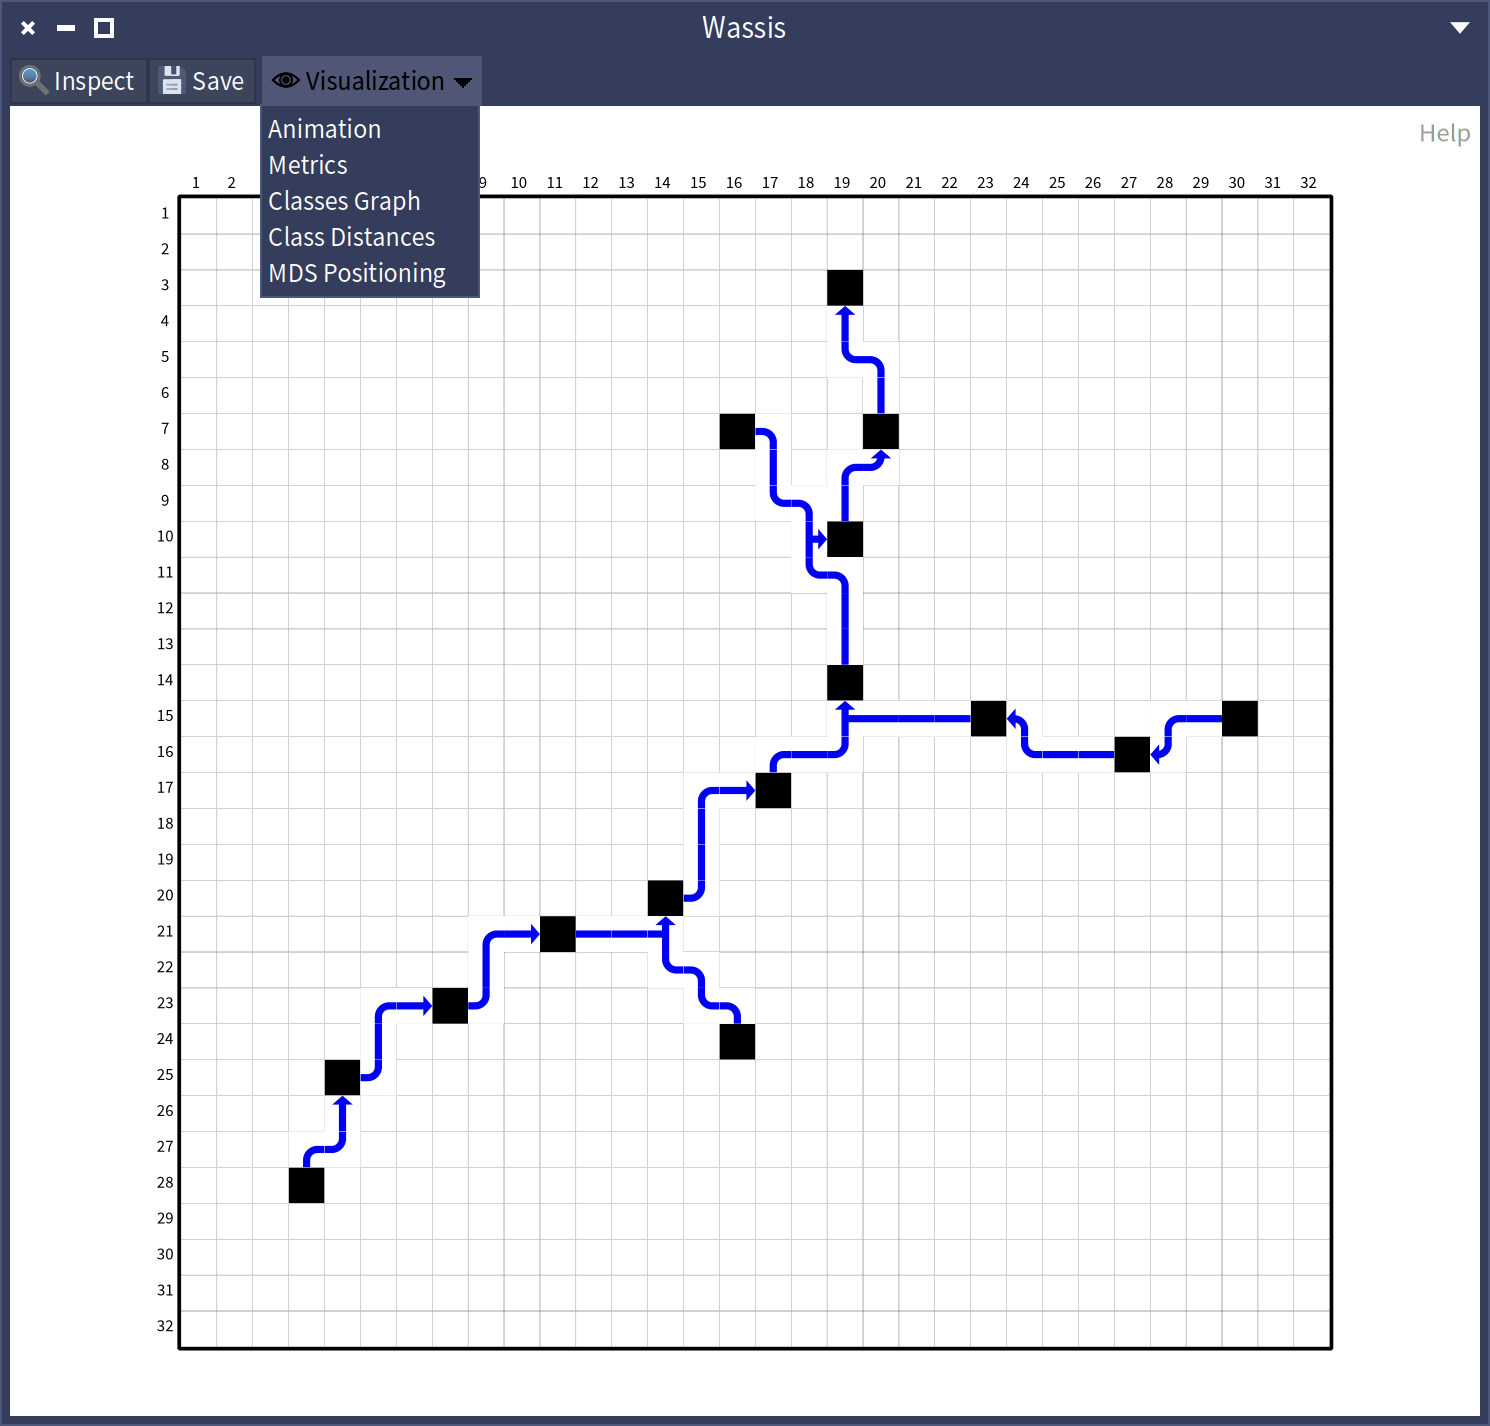
\includegraphics[width=0.75\textwidth]{figures/implementation/tool/visualization}
    \caption{Main grid visualization.}
    \label{fig:visualization}
\end{figure}

The additional views include the step-by-step animation, the metrics dashboard, the system graph, the distance matrix, and the MDS placement. 

\subsection{Step-by-Step Animation}

\wassis provides a step-by-step animation to inspect the WFC generation process (\figref{fig:animation}). The animation shows the state of the grid at each step, from start to finish. The \texttt{Reset}, \texttt{Step Back}, \texttt{Play}, and \texttt{Step Forward} buttons allow users to move through the generation process, along with the slider.

\begin{figure}[ht]
    \centering
    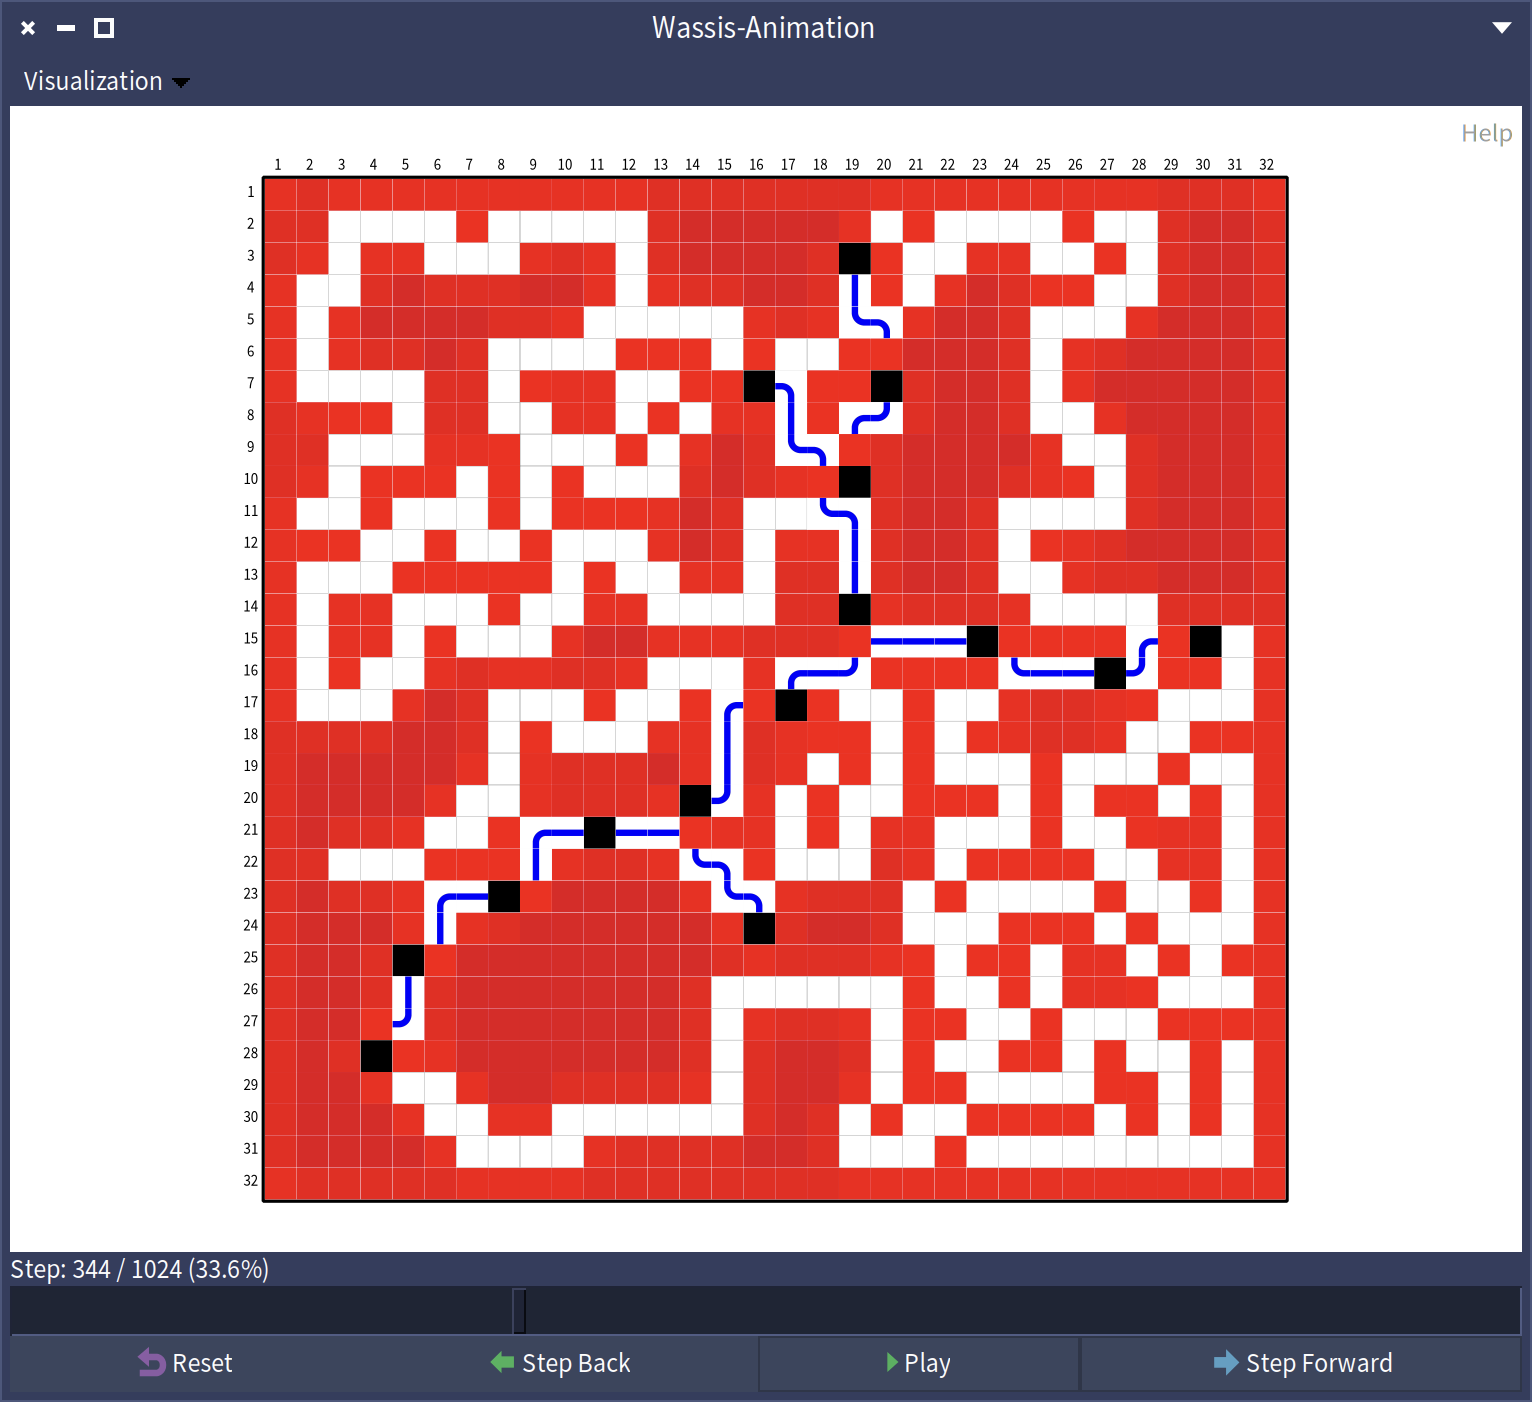
\includegraphics[width=0.75\textwidth]{figures/implementation/tool/animation}
    \caption{WFC step-by-step animation window.}
    \label{fig:animation}
\end{figure}

\subsection{Metrics Dashboard}

\wassis includes a metrics dashboard with several tabs. Each tab provides information about a different part of the generated layout and the WFC execution:

\begin{itemize}
    \item \textbf{Graph Metrics} (\figref{fig:graph_metrics}): Shows the grid size, the number of class cells, path cells, and empty cells in the grid, as well as the number of overlaps.
     
    \item \textbf{Performance Metrics} (\figref{fig:performance_metrics}): Shows the total execution time, the WFC solving time, and the number of attempts needed to find the solution. The total execution time is measured from the moment the user clicks \texttt{Run} until the final visualization is displayed. The WFC solving time refers only to the time spent by WFC to generate the solution in the successful attempt.
   
    \item \textbf{Placement Metrics} (\figref{fig:placement_metrics}): Shows the average distance between each class and its connected classes, as well as the pairwise distances between classes on the grid, computed using Manhattan distance.
    
    \item \textbf{System Metrics} (\figref{fig:system_metrics}): Shows the total number of classes, the average number of connections per class, and the number of connections of each class.
\end{itemize}

\begin{figure}[ht]
    \centering
    \begin{subfigure}{\textwidth}
        \centering
        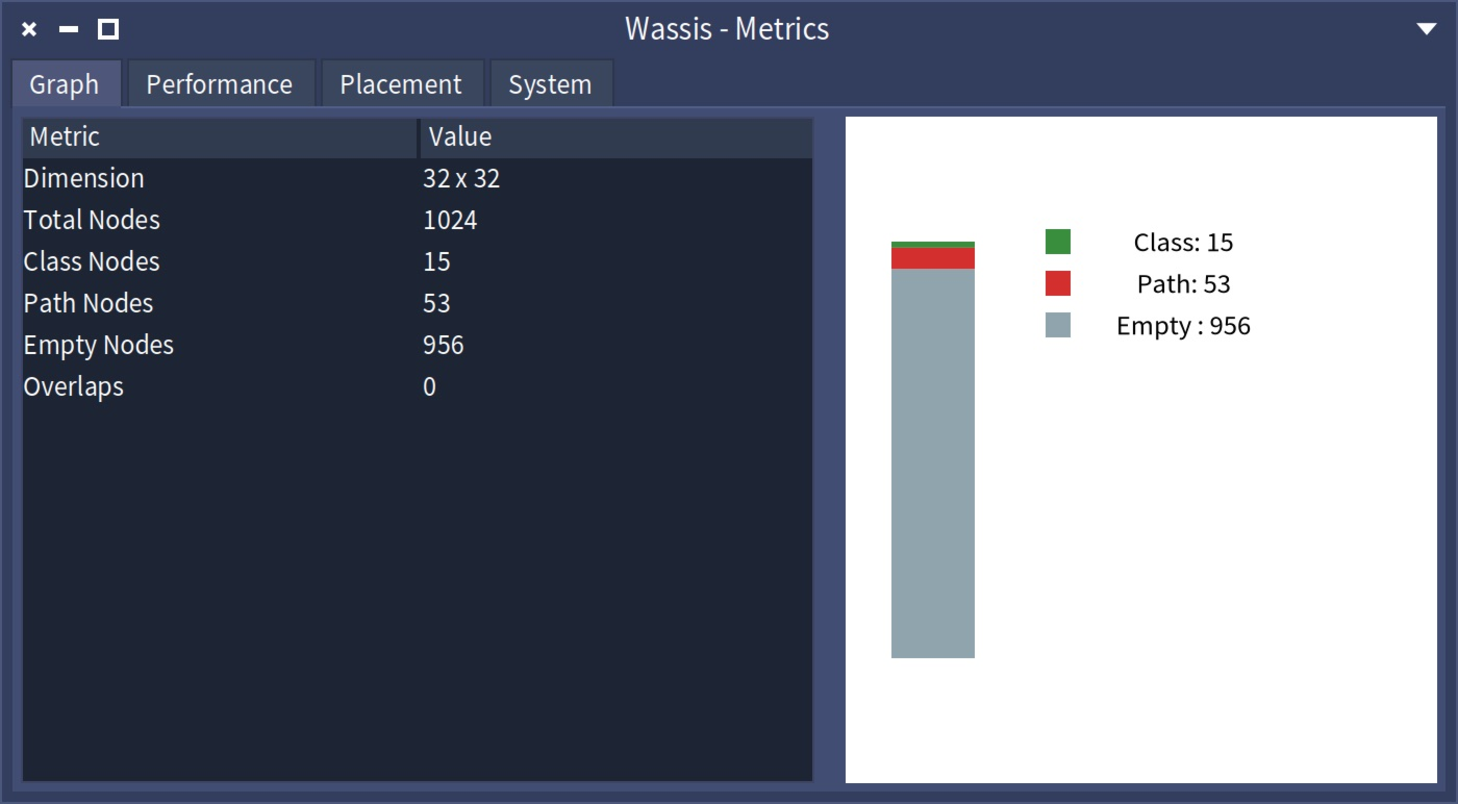
\includegraphics[height=0.2309\textheight, keepaspectratio]{figures/implementation/tool/graph_metrics}
        \caption{Graph metrics panel.}
        \label{fig:graph_metrics}
    \end{subfigure}
    \vspace{2pt}
    \begin{subfigure}{\textwidth}
        \centering
        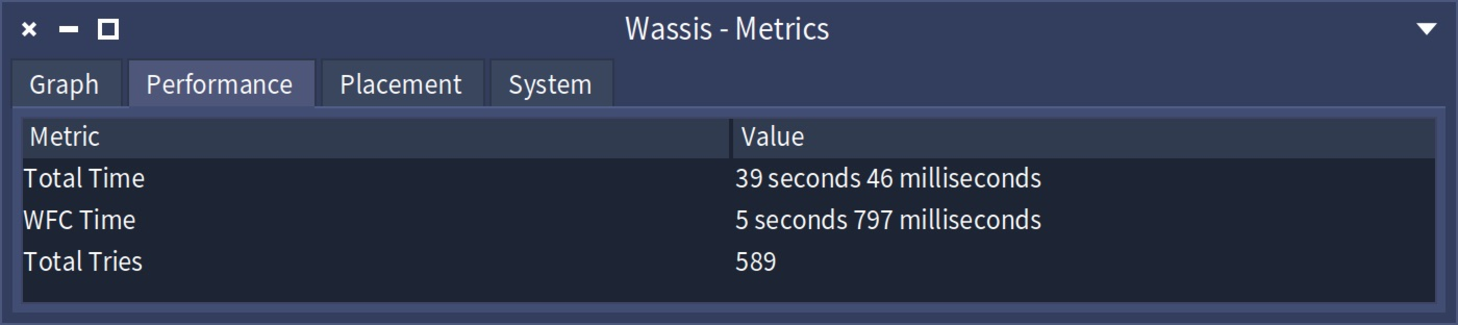
\includegraphics[height=0.0932\textheight, keepaspectratio]{figures/implementation/tool/performance_metrics}
        \caption{Performance metrics panel.}
        \label{fig:performance_metrics}
    \end{subfigure}
    \vspace{2pt}
    \begin{subfigure}{\textwidth}
        \centering
        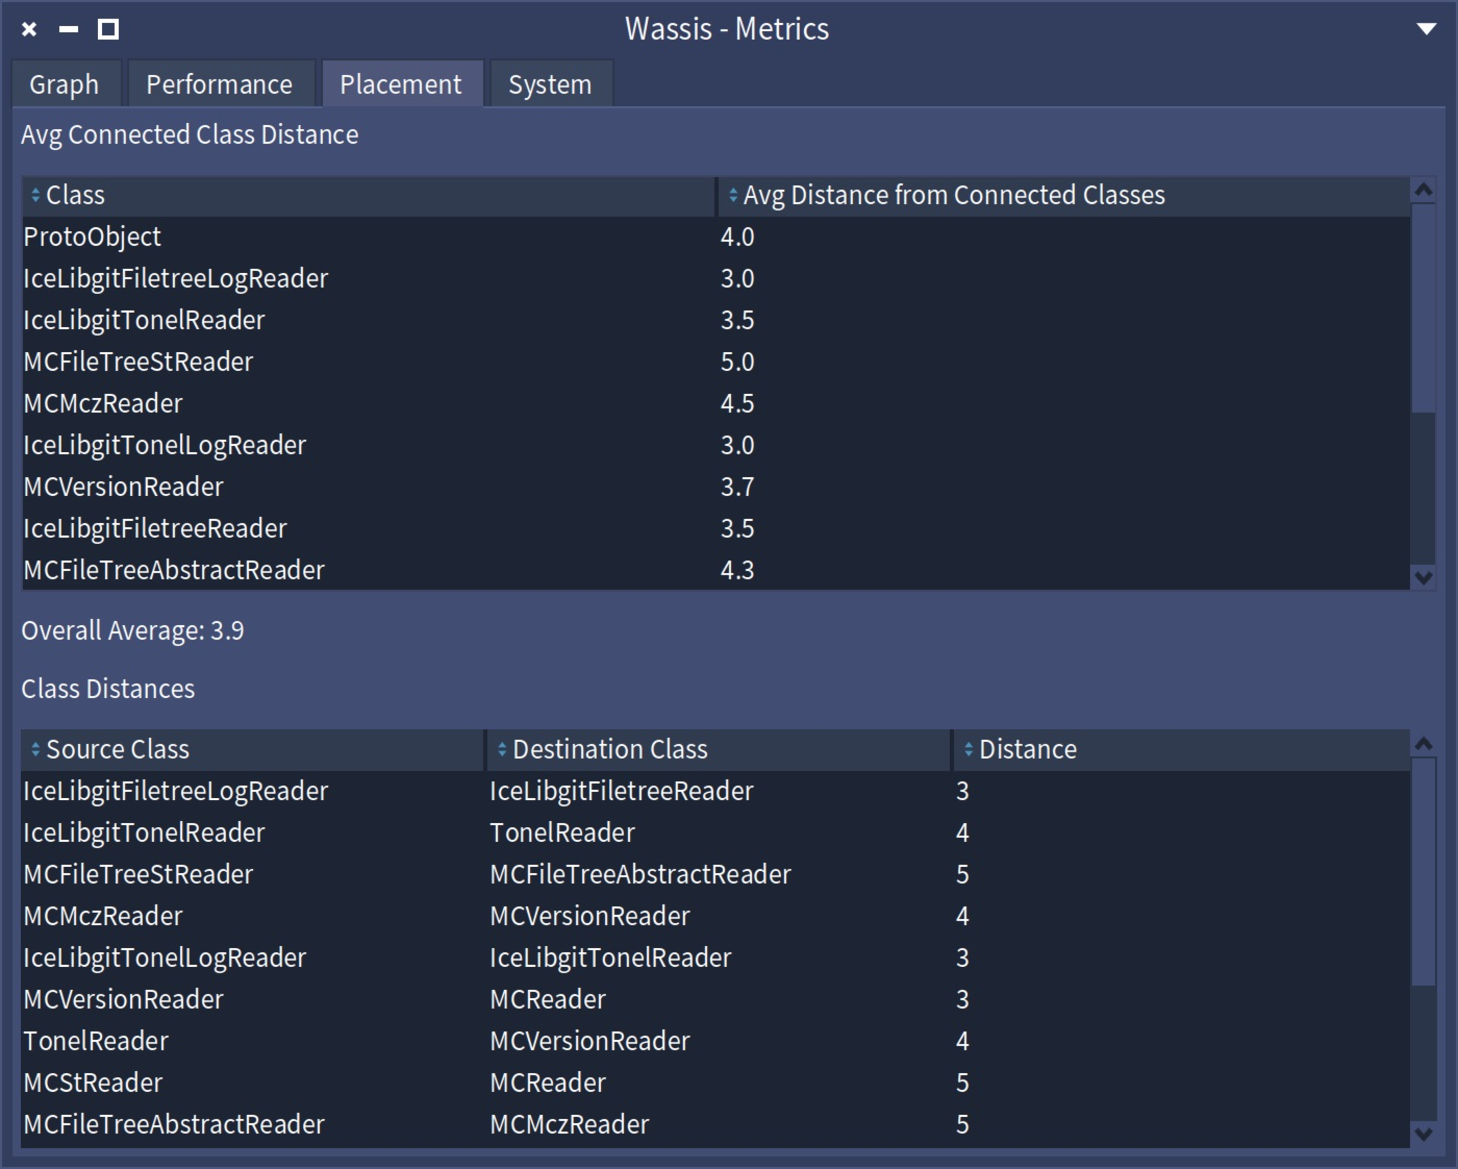
\includegraphics[height=0.335\textheight, keepaspectratio]{figures/implementation/tool/placement_metrics}
        \caption{Placement metrics panel.}
        \label{fig:placement_metrics}
    \end{subfigure}
    \vspace{2pt}
    \begin{subfigure}{\textwidth}
        \centering
        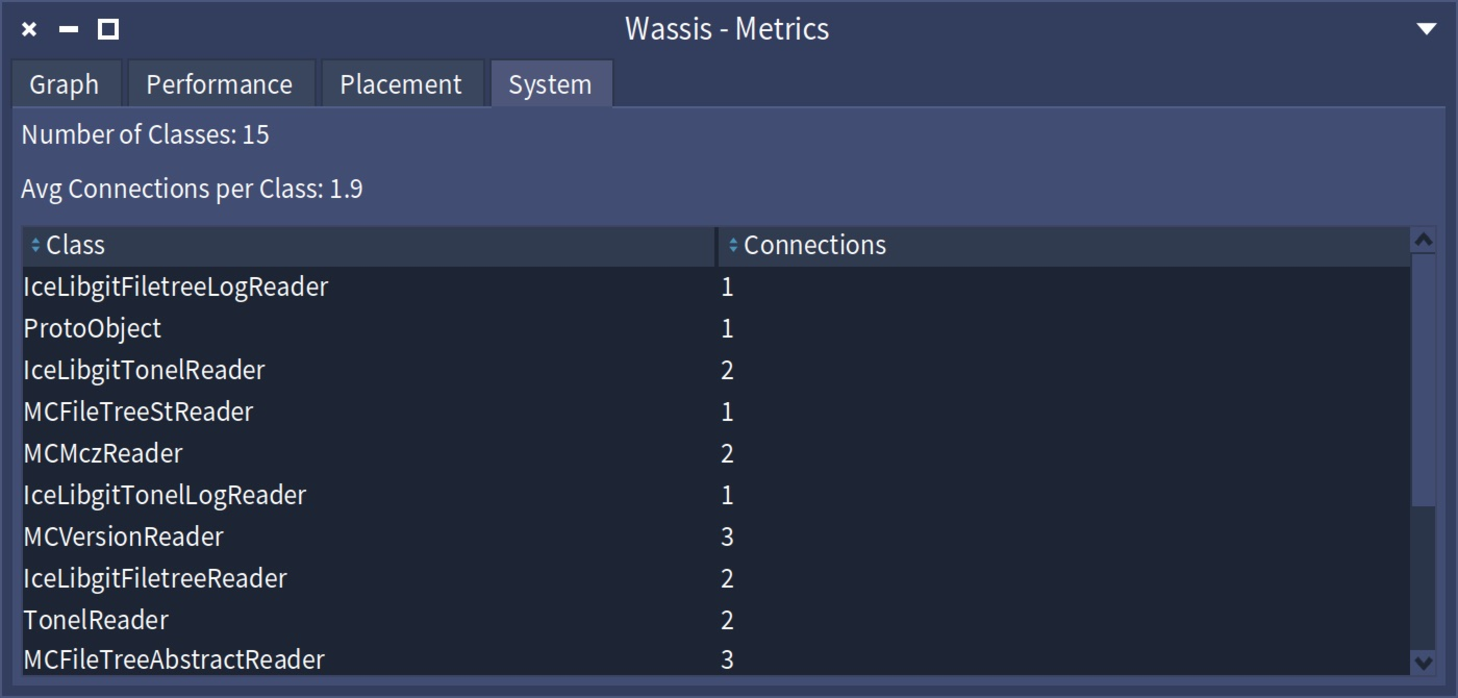
\includegraphics[height=0.20\textheight, keepaspectratio]{figures/implementation/tool/system_metrics}
        \caption{System metrics panel.}
        \label{fig:system_metrics}
    \end{subfigure}
    \caption{Overview of the tool metrics panels.}
    \label{fig:tool_metrics_panels}
\end{figure}

% \subsection{System Graph}
% The system can also be displayed using a force-directed graph (\figref{fig:classes_graph}) to compare this visualization with the one generated using \wassis.

% \begin{figure}[ht]
%     \centering
%     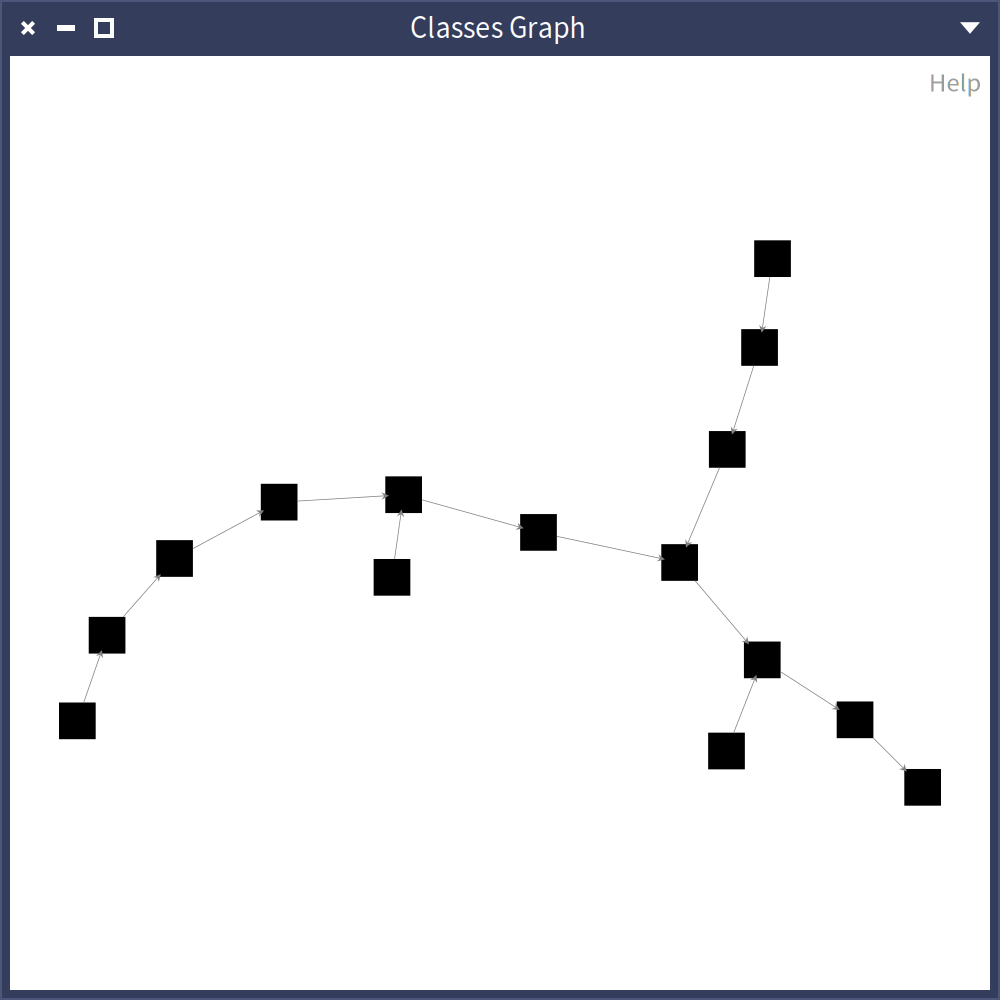
\includegraphics[width=0.8\textwidth]{figures/implementation/tool/classes_graph}
%     \caption{Force-direct graph of the system.}
%     \label{fig:classes_graph}
% \end{figure}

\end{document}